\documentclass[12pt,a4paper]{report}

%Set language
\usepackage[english]{babel}
\usepackage{enumerate}

% To import and adjust images
\usepackage{graphicx}
\usepackage[export]{adjustbox}
\usepackage[center]{caption}
\usepackage{subcaption}
\usepackage{float}
\usepackage{tabularx}

% To build a clickable Toc
\usepackage{color} %May be necessary if you want to color links
\usepackage{hyperref}
\hypersetup{
    colorlinks=true, %set true if you want colored links
    linktoc=all,     %set to all if you want both sections and subsections linked
    linkcolor=black,  %choose some color if you want links to stand out
    urlcolor = black
}

%To load PoLitecnico's logo
\usepackage{titling}

% Command to hide subsections in the Toc
\setcounter{tocdepth}{1}

% I don't like dots in the Toc
\usepackage{tocloft}
\renewcommand{\cftdot}{}


% Path relative to the .tex file containing the \includegraphics command
\graphicspath{ {./images/} }  

% To change the ToC title
\addto\captionsenglish{ \renewcommand {\contentsname} {Table of
contents}}

%logo 
\pretitle{
	 \begin{center}
	 \LARGE
	 
\includegraphics[width = 0.6\textwidth]{logo}\\[\bigskipamount]
}
\posttitle{\end{center}}

% Here we go
\title{SafeStreets - DD \\ \large version 1.0}
\author{Frangi Alberto, Fucci Tiziano}
\date{A.Y. 2019/2020}
\begin{document}
	\maketitle
	%Index
	\tableofcontents 
	\chapter{Introduction}
		\section{Purpose}
			The purpose of this document consists of giving more technical details than the RASD concerning the SafeStreets
			system.\\
			The RASD document completely describes the system in terms of functional and nonfunctional requirements and
			serves as a contractual basis between the customer and the developer and it must be written in the language of
			the customer's domain of business/expertise, the DD's purpose instead is to provide a description for how the new
			system will be constructed, it provides a description of the system architecture, software, hardware, database
			design, and security.\\
			In particular this document will explain the following topics:
			\begin{itemize}
				\item High level architecture and its components' requirements;
				\item Run-time behavior;
				\item Design patterns;
				\item Additional user interfaces information;
				\item Implementation, integration and testing plan.
			\end{itemize}
		\section{Scope}
			Safestreet is an application to be used both from civilians (users) and authorities, in order to help the latter and
			reduce traffic violations. Registered authorities can automatically receive reports made by users, so the service acts
			as an intermediary. The next paragraph gives a more formal description of system's architecture.

		\section{Definitions, Acronyms, Abbreviations}
			\subsection{Definitions}
				\begin{itemize}
				\item \textbf{User}: a civilian customer that can use the application to:
					\begin{itemize}
					\item notify authorities of some violation;
					\item check which are the most dangerous (i.e. with the most violations) streets.
					\end{itemize}
				In this document, ``user", ``citizen" and ``civiian" are completely equivalent, where not specified.
				\item \textbf{Authority}: a member of the local police who has access to reports made by users. The
					authorities evaluate the reports sent by the user to determine if the violation stands.
				\item \textbf{Report}: a message consisting of:
					\begin{itemize}
					\item a picture showing the car in order to show the occurring violation;
					\item date and time of the picture;
					\item GPS position of the place where the violation occurred;
					\item the street where the violation occurred (automatically retrieved from the geographical position);
					\item the type of the violation (input by the user)
					\end{itemize}
				\item \textbf{Available}: a report is available for an authority if its position is within the municipality assigned
					to the authority.
				\item \textbf{Violation}: a situation that, according to the user who sent the report, is a violation of the
					traffic laws.
				\item \textbf{Intervention}: a brief text suggesting a possible solution in order to improve safety and
					discourage future violations.
				\end{itemize}
			\subsection{Acronyms}
				\begin{itemize}
				\item \textbf{API}: \emph{Application Programming Interface.}
				\item \textbf{GPS}: \emph{Global Positioning System.}
				\item \textbf{UI}: \emph{User Interface.}
				\item \textbf{RASD:} \emph{Requirements Analysis and Specifications Document}
				\item \textbf{DD:} \emph{Design Document}
				\item \textbf{DMZ:} \emph{DeMilitarized Zone}			
				\item \textbf{PKC}: \emph{Public Key Cryptography.}		
				\item \textbf{AES}: \emph{Advanced Encryption Standard.}		
				\end{itemize}
		\section{Revision History}
			\begin{itemize}
				\item \textbf{Version 1.0:} 
				\begin{itemize}
					\item First release.
				\end{itemize}
			\end {itemize}
		\section{Reference Documents}
			\begin{itemize}
				\item \textbf{Specification document:} "Mandatory project assignment AY 2019/20".
			\end{itemize}
		\section{Document Structure}
			\begin{itemize}
				\item \textbf{Chapter 1} provides a brief explanation on the DD purpose and a quick introduction
					SafeStreets.
				\item \textbf{Chapter 2} aims to provide a description of the system's architecture. 
				\item \textbf{Chapter 3} specifies the design of user interfaces and describes the user-application
					interaction.
				\item \textbf{Chapter 4} contains requirements traceability.
				\item \textbf{Chapter 5} describes the implementation plan.
				\item \textbf{Chapter 6} shows the effort of each group member.
				\item \textbf{Chapter 7} contains all the references used to make this document. 
			\end{itemize}
	%end of first chapter
	
	\chapter{Architectural design}
		\section{Overview:	high-level	components	and	their	interaction} 
	The application is built following the principles of the three-tier architecture: the three logic layers of presentation, 				application and data access rely on three corresponding hardware layers. This architecture is prefered to one-tier and 			two-tier architectures due to some important characteristics, some of which are:
	\begin{itemize}
	\item \emph{Flexibility:} each tier can be manged or scaled independently at any time, without affecting the others;
	\item \emph{Scalability:} following a scale-out approach, performances can be improved through node replication, without affecting the other tiers.
	Load balancing systems distribute the working load among the nodes;
	\item \emph{Mantainability:} because each tier is independent from the others, updates or changes can be released
	without affecting the whole system;
	\item \emph{Availbility:} with this architecture, it is less likely to have failures that compromise the whole application.
	Load balancing and node replication minimize the performance loss when a failure occures.
	\end{itemize}
	A general view of the system architecture is provided in the following picture:
	\begin{figure}[H]
				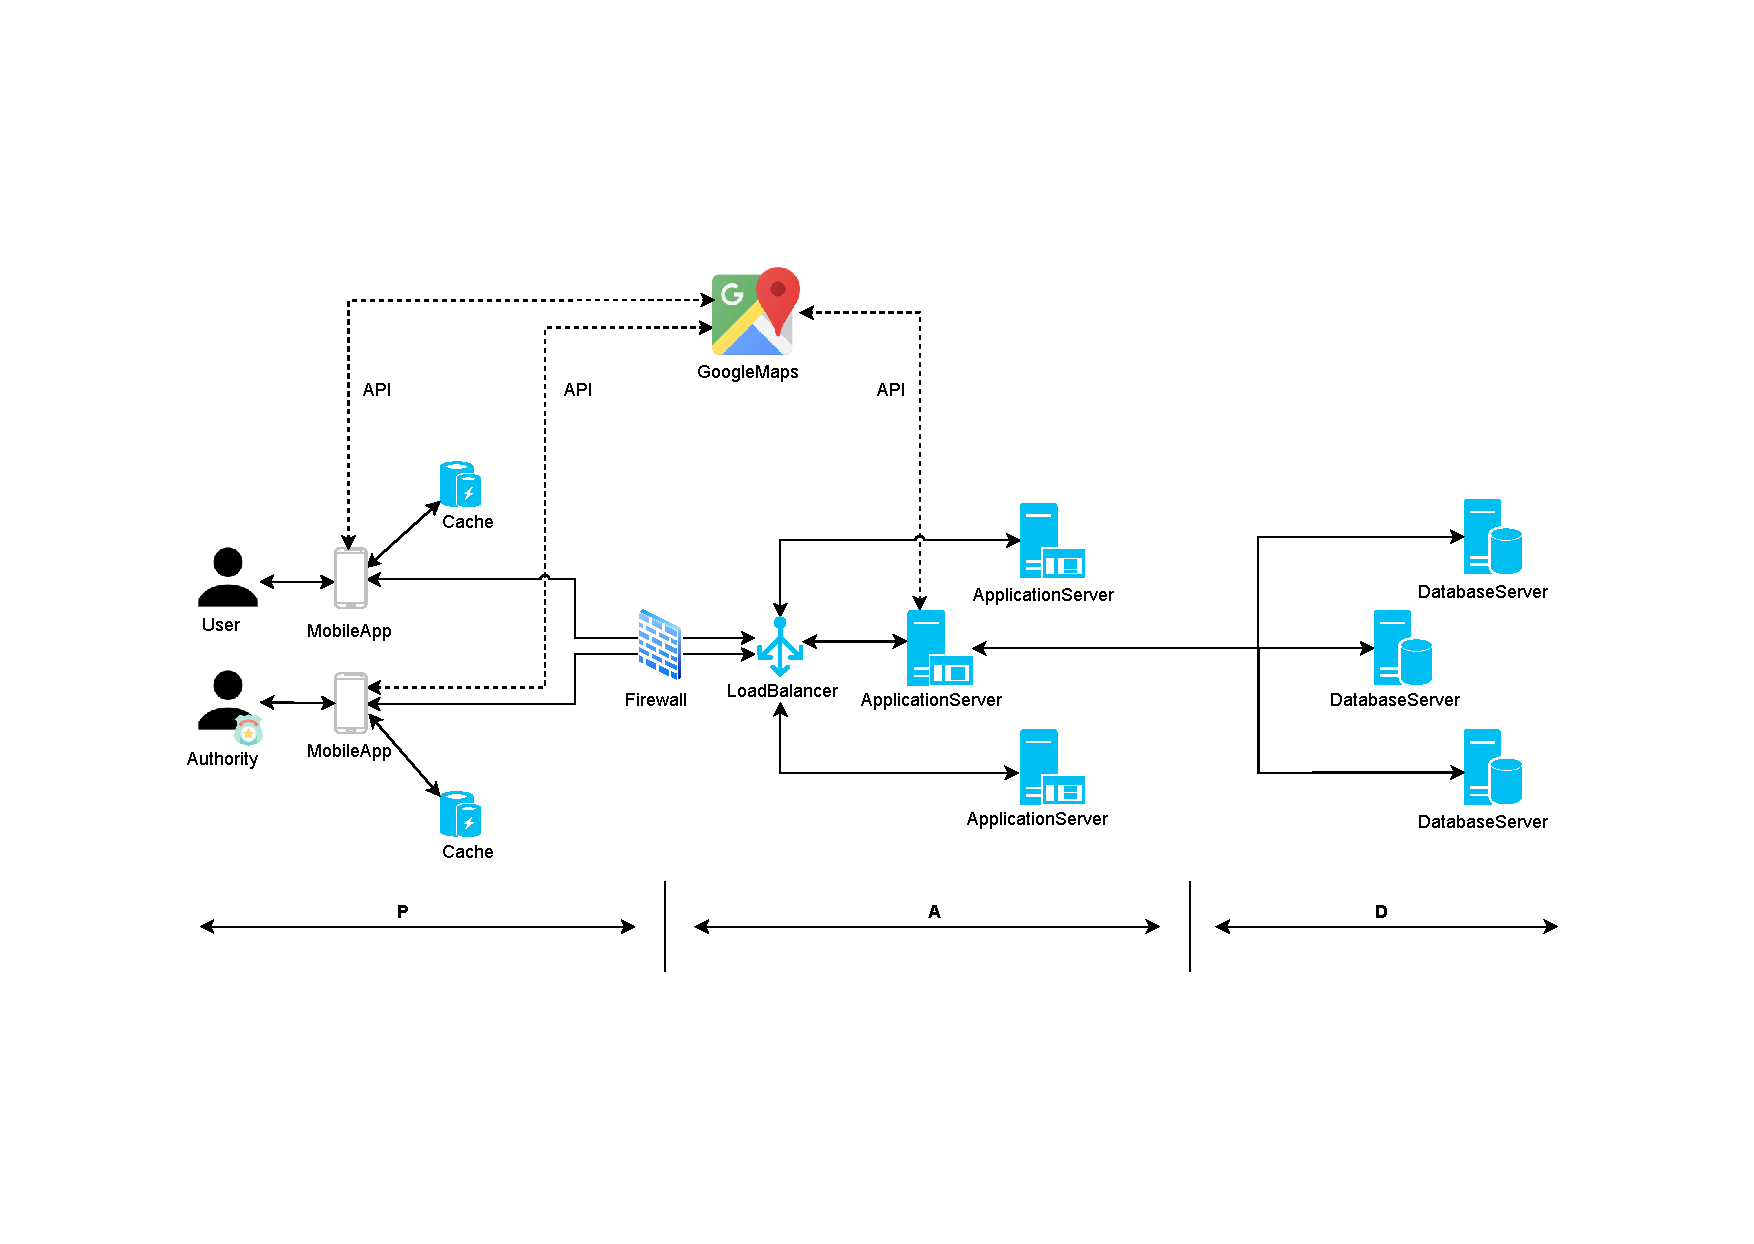
\includegraphics[scale = 0.6, center]{sysarch}
				\caption{System architecture}
		\end{figure}
	Users and authorities are provided with mobile devices and access the service through
	the SafeStreets mobile app. The mobile app communicates with the application layer, which
	is made by one or more application servers, linked to the database servers. The scale-out approach allows to adjust the number of hardware resources at any time. For what concerns the data access layer, database servers contain sensitive information, such as password hashes, license plate numbers, identification numbers and so on, so it is important to protect all the back-end of the application. In order to do this, the application and data access levels are protected by a firewall that performs traffic control at the level of the single packet, creating a DMZ in which the communication is safe.

		\section{Component view}
		\section{Deployment view}
		\section{Runtime view}
			\subsection{Making report}					
				\begin{figure}[H]
						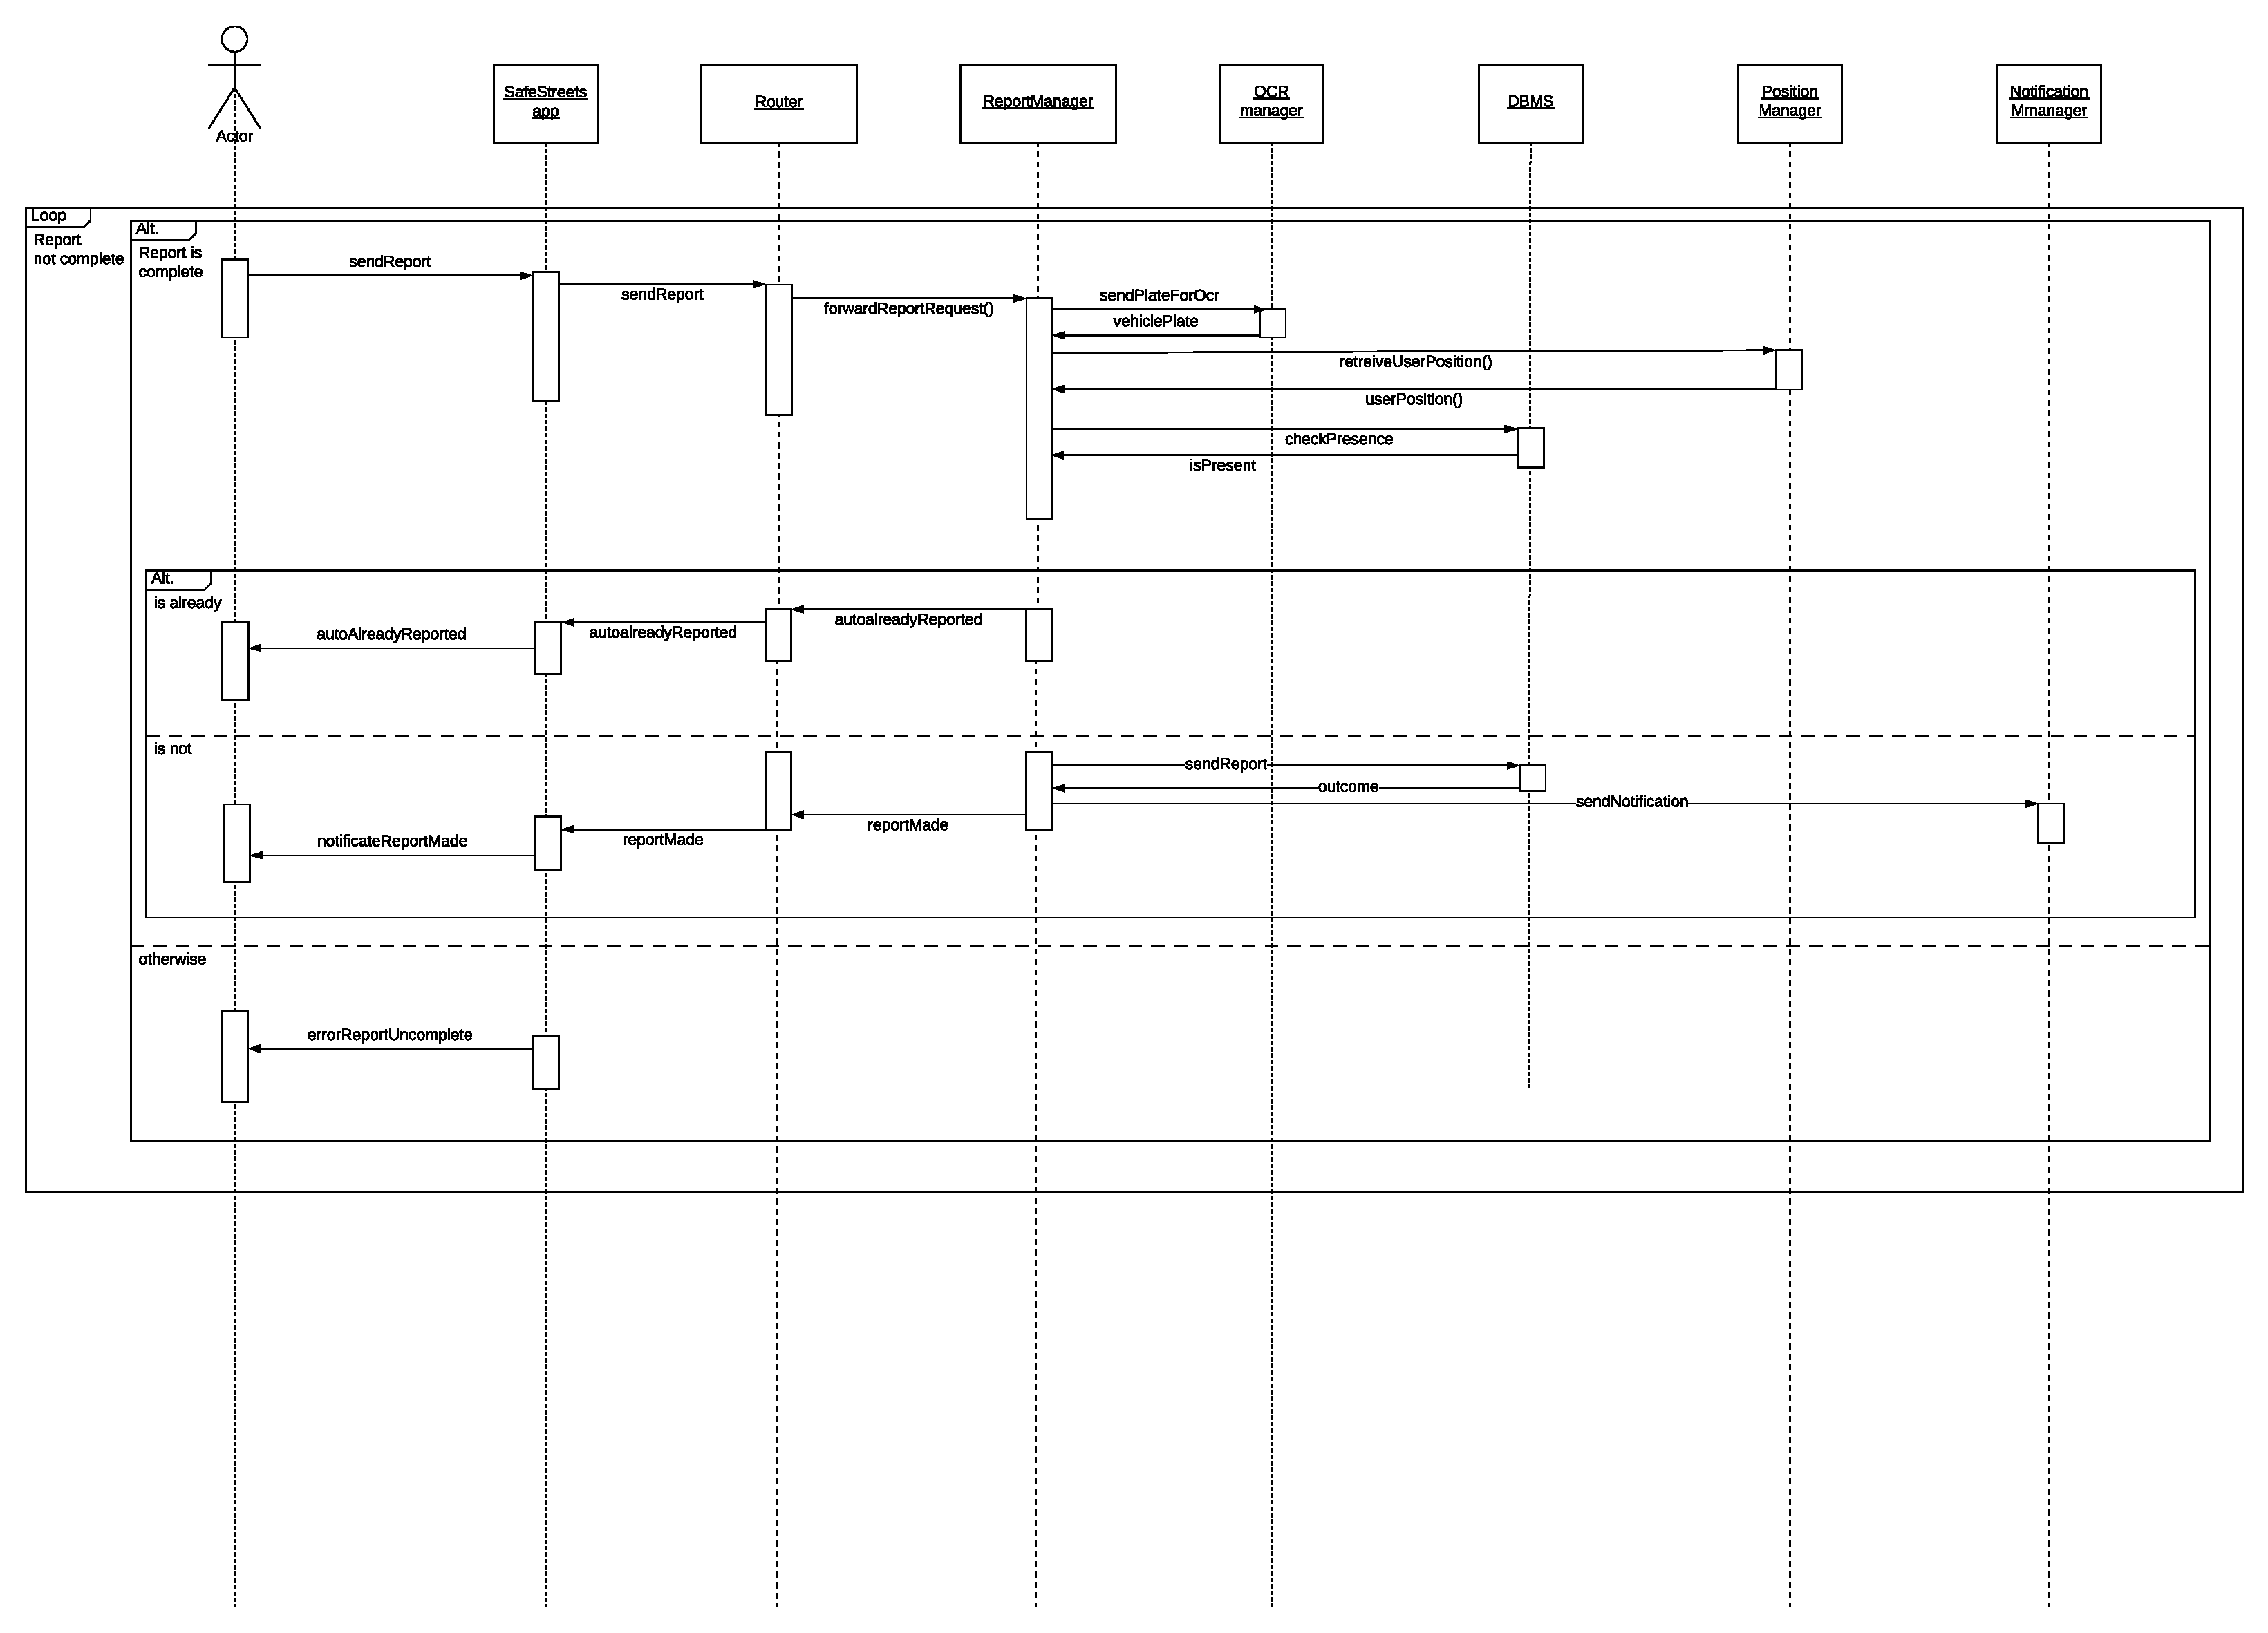
\includegraphics[width = 1.5\textwidth, center]{Report}
						\caption{}
				\end{figure}
			\subsection{Visualize Maps}					
				\begin{figure}[H]
						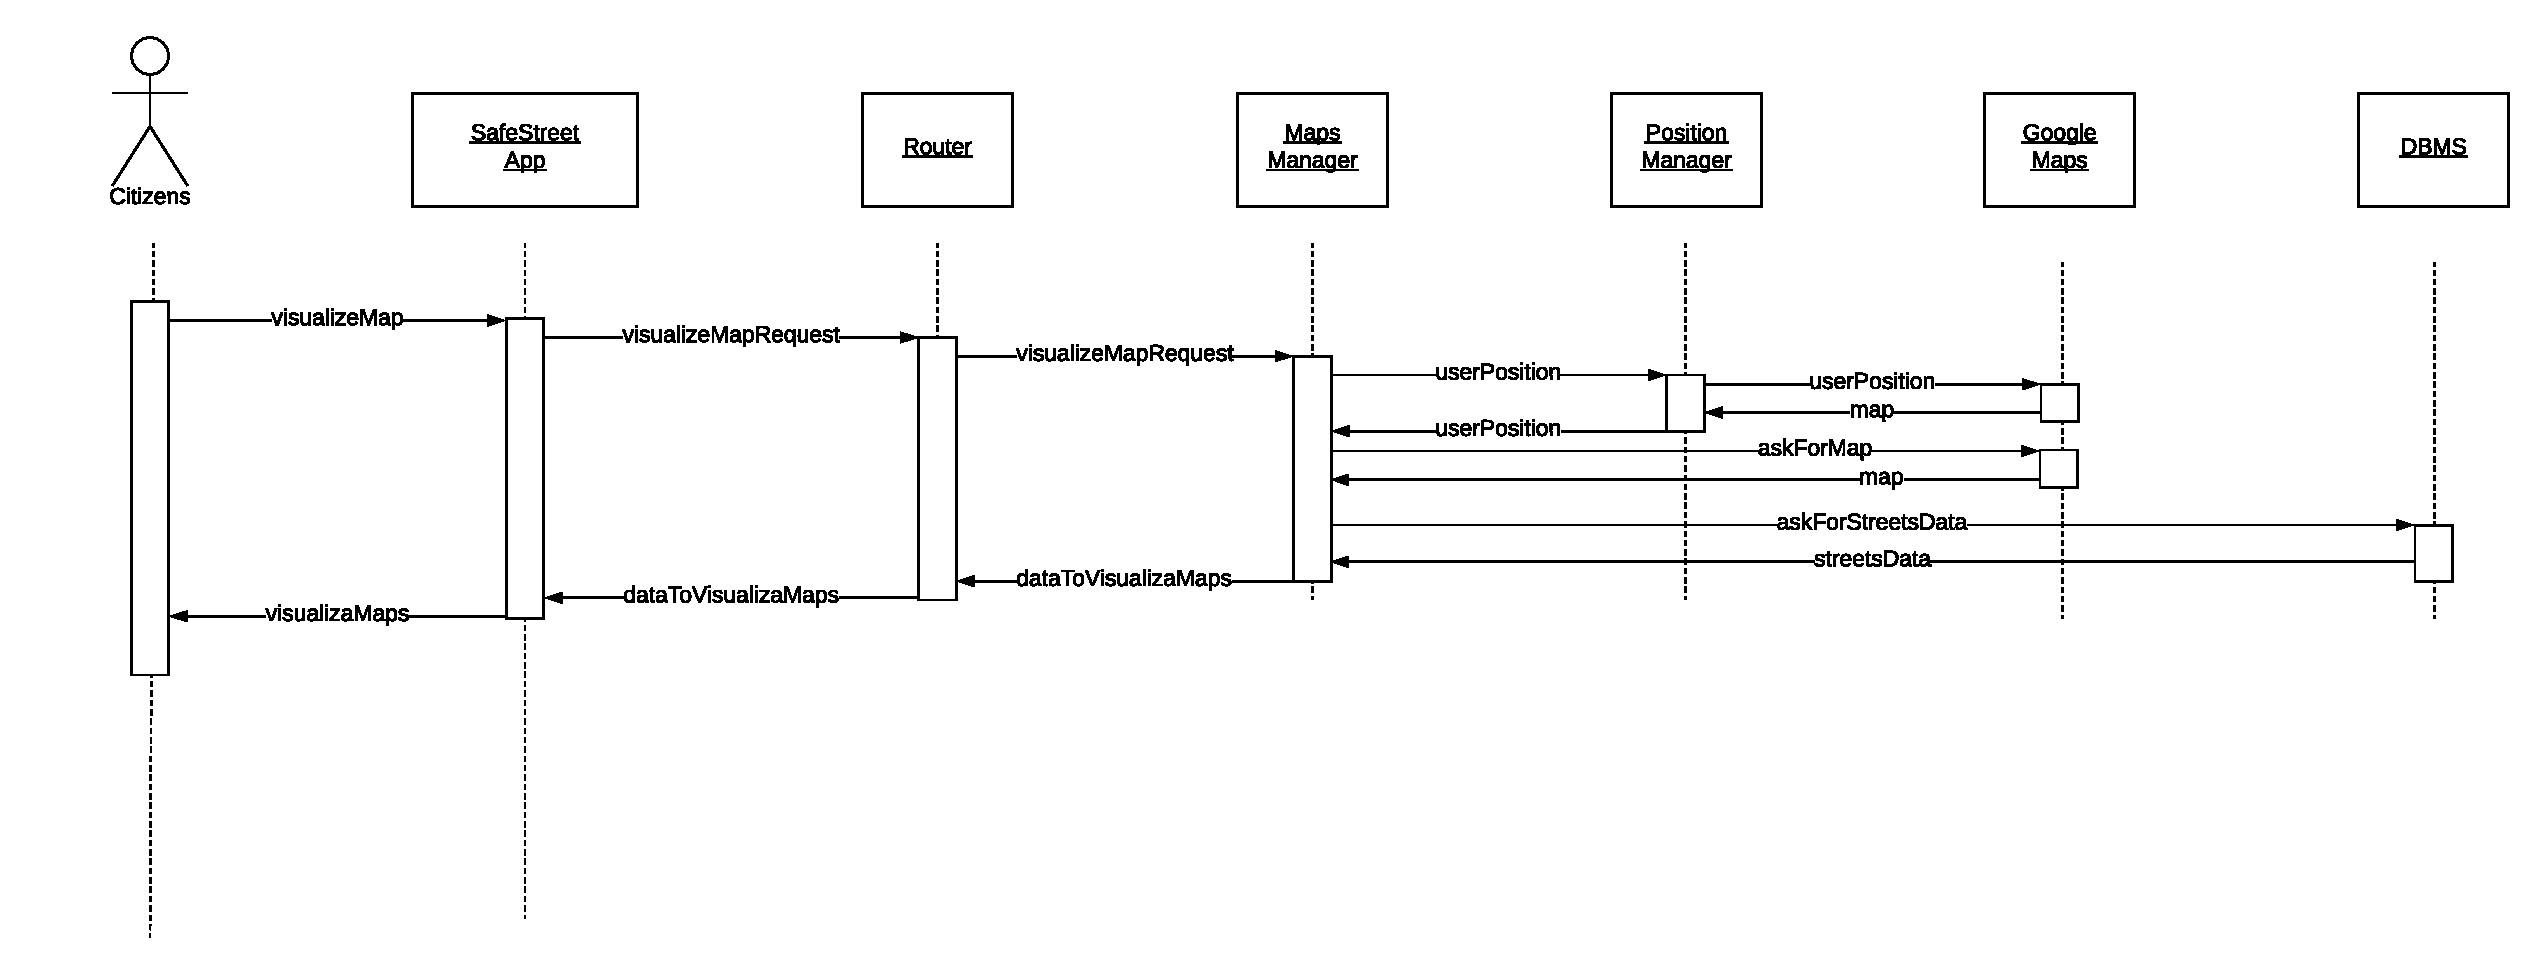
\includegraphics[width = \textwidth, center]{Maps}
						\caption{}
				\end{figure}
			\subsection{Visualize reports' history}					
				\begin{figure}[H]
						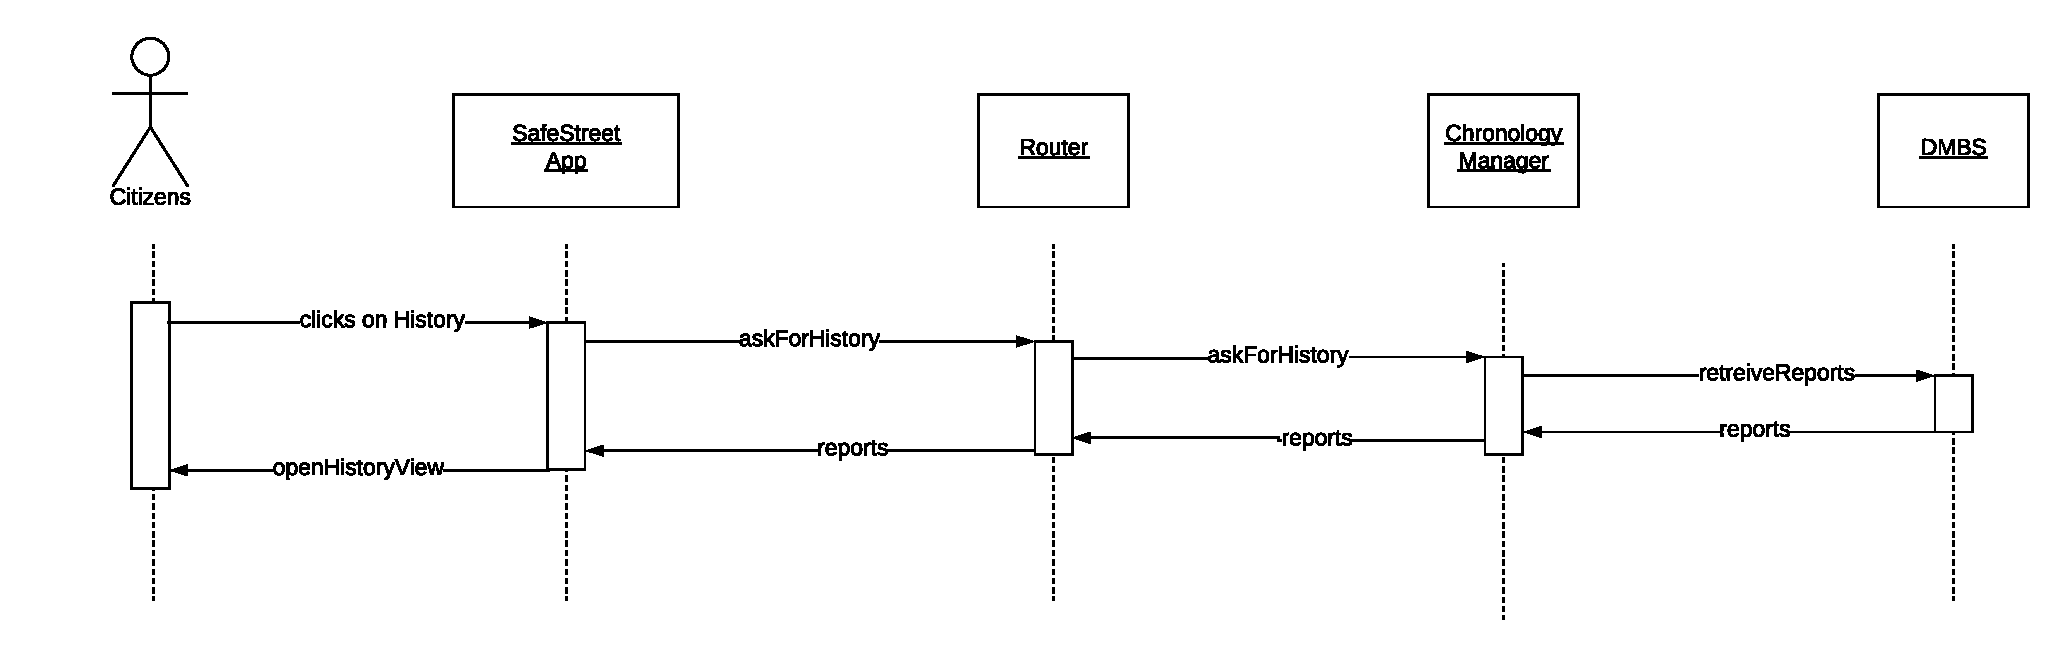
\includegraphics[width = \textwidth, center]{history}
						\caption{}
				\end{figure}
			\subsection{Evaluate report}					
				\begin{figure}[H]
						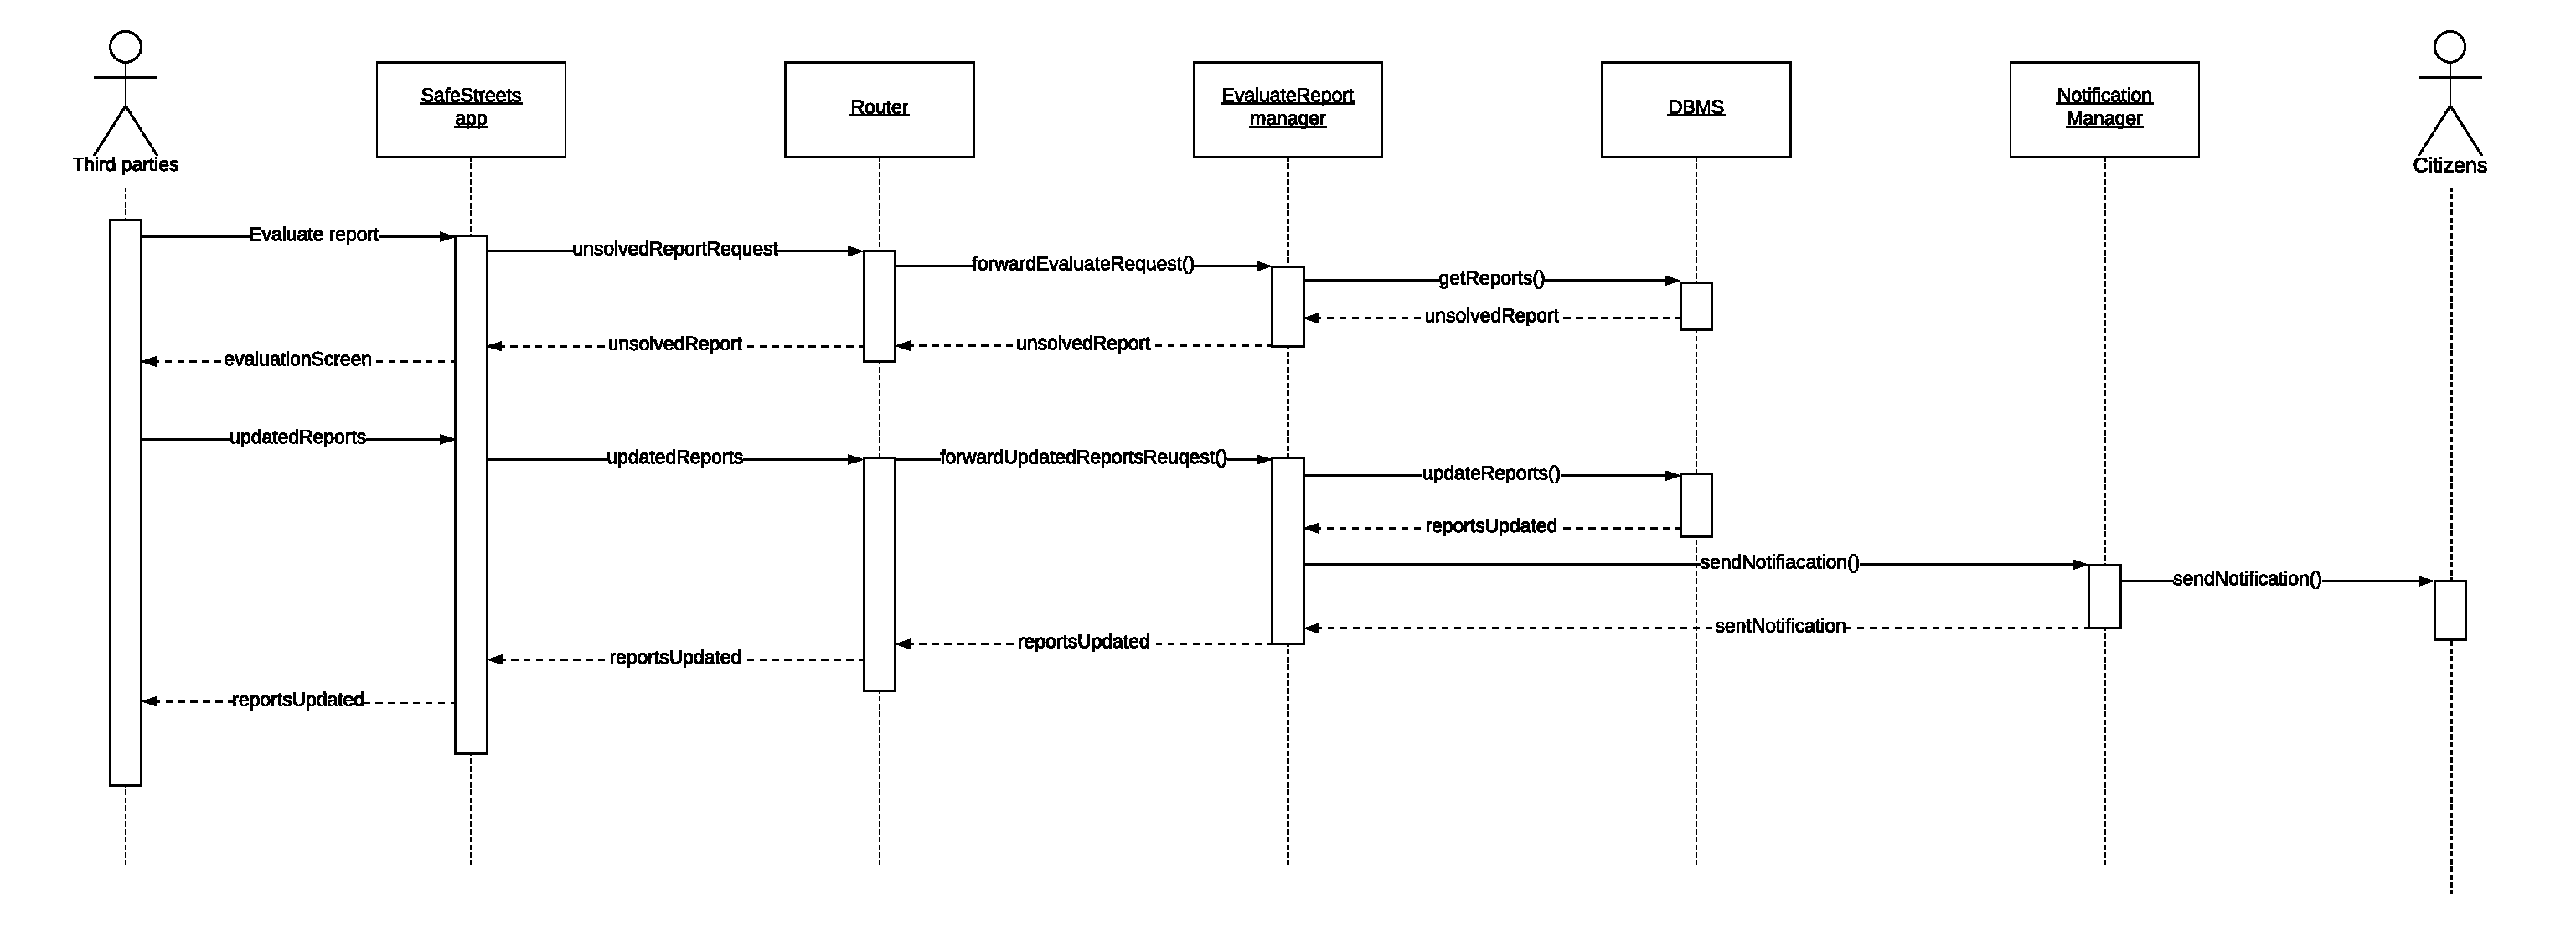
\includegraphics[width = \textwidth, center]{Evaluate}
						\caption{}
				\end{figure}
		\section{Component interfaces}
		\section{Selected architectural styles and patterns}
		\section{Other design decisions}
	%end of second chapter
	
	\chapter{User interfaces design}
	\section{User}
		\begin{figure}[H]
				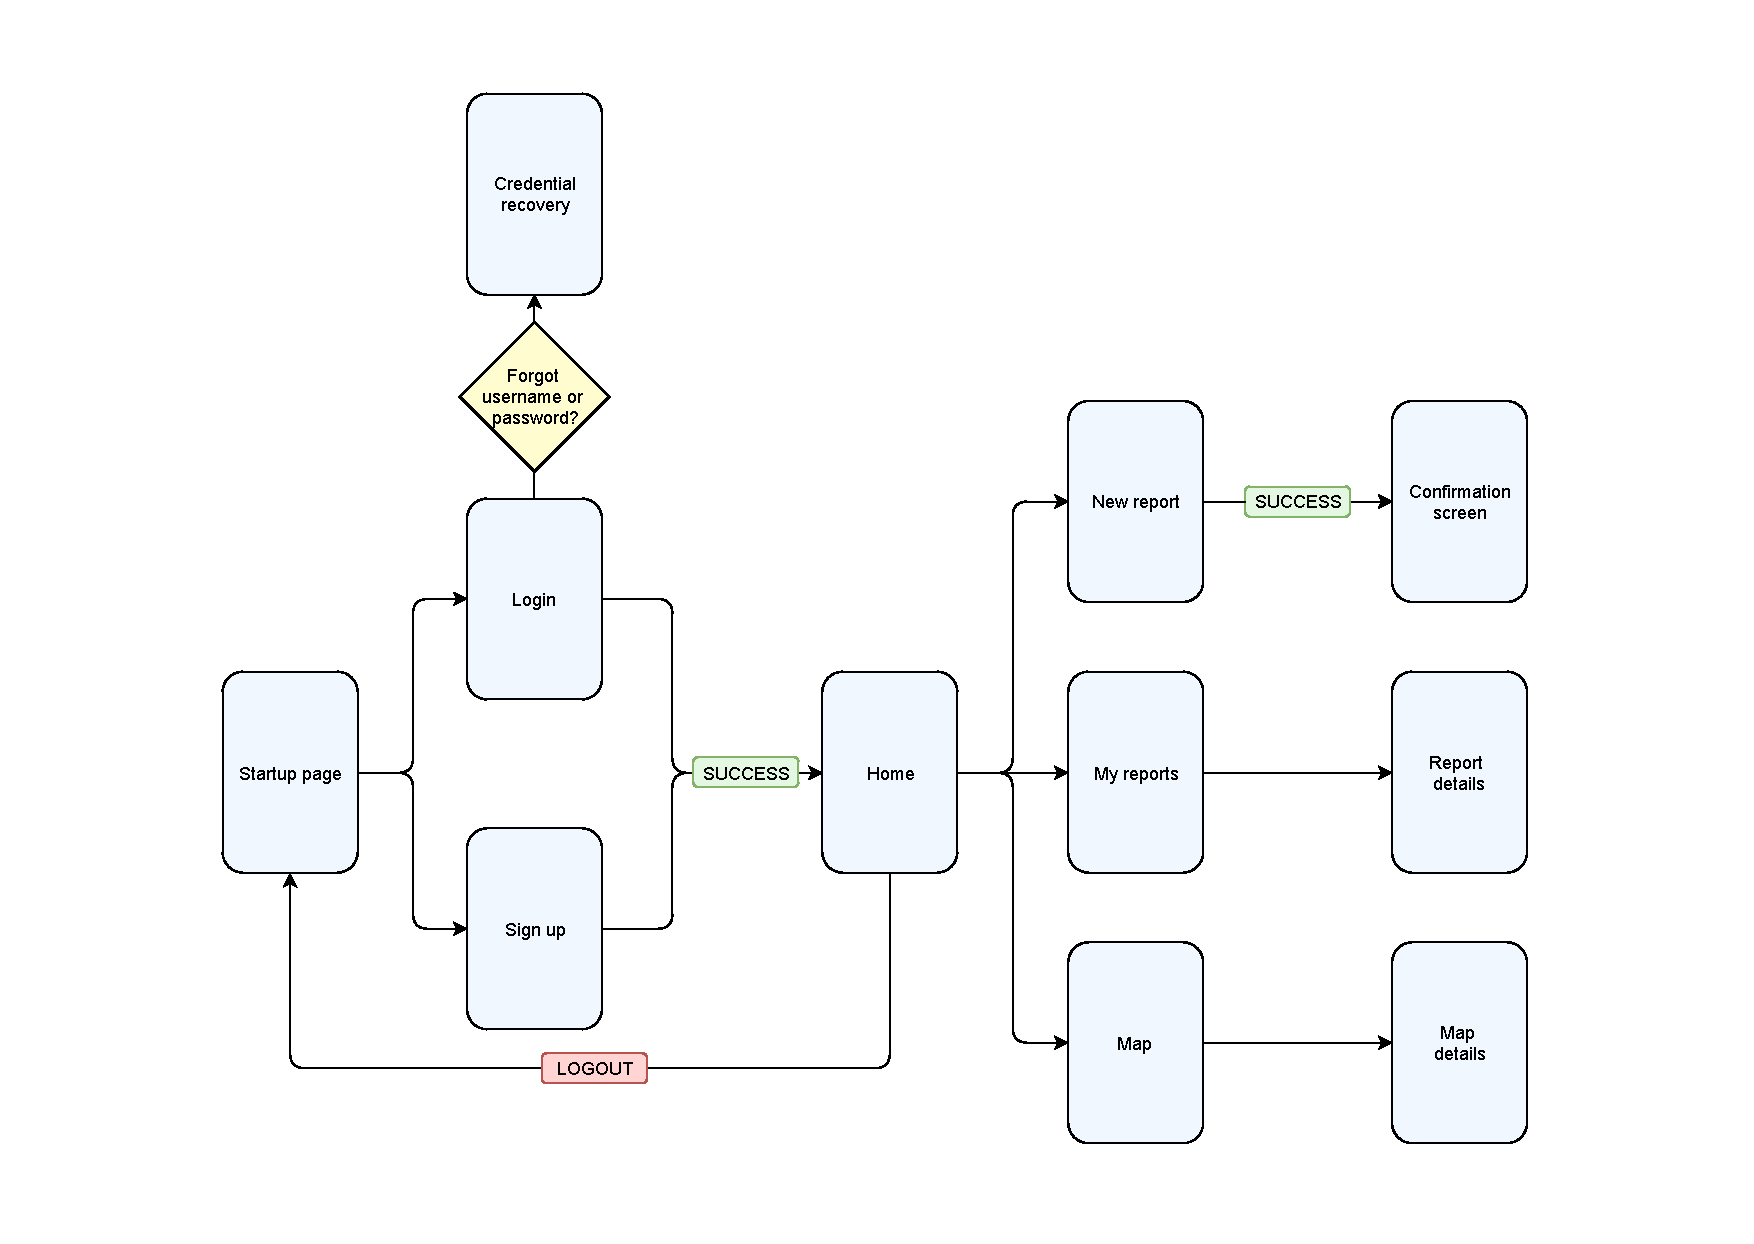
\includegraphics[scale = 0.6, center]{userux}
				\caption{}
		\end{figure}
	\section{Authority}		
		\begin{figure}[H]
				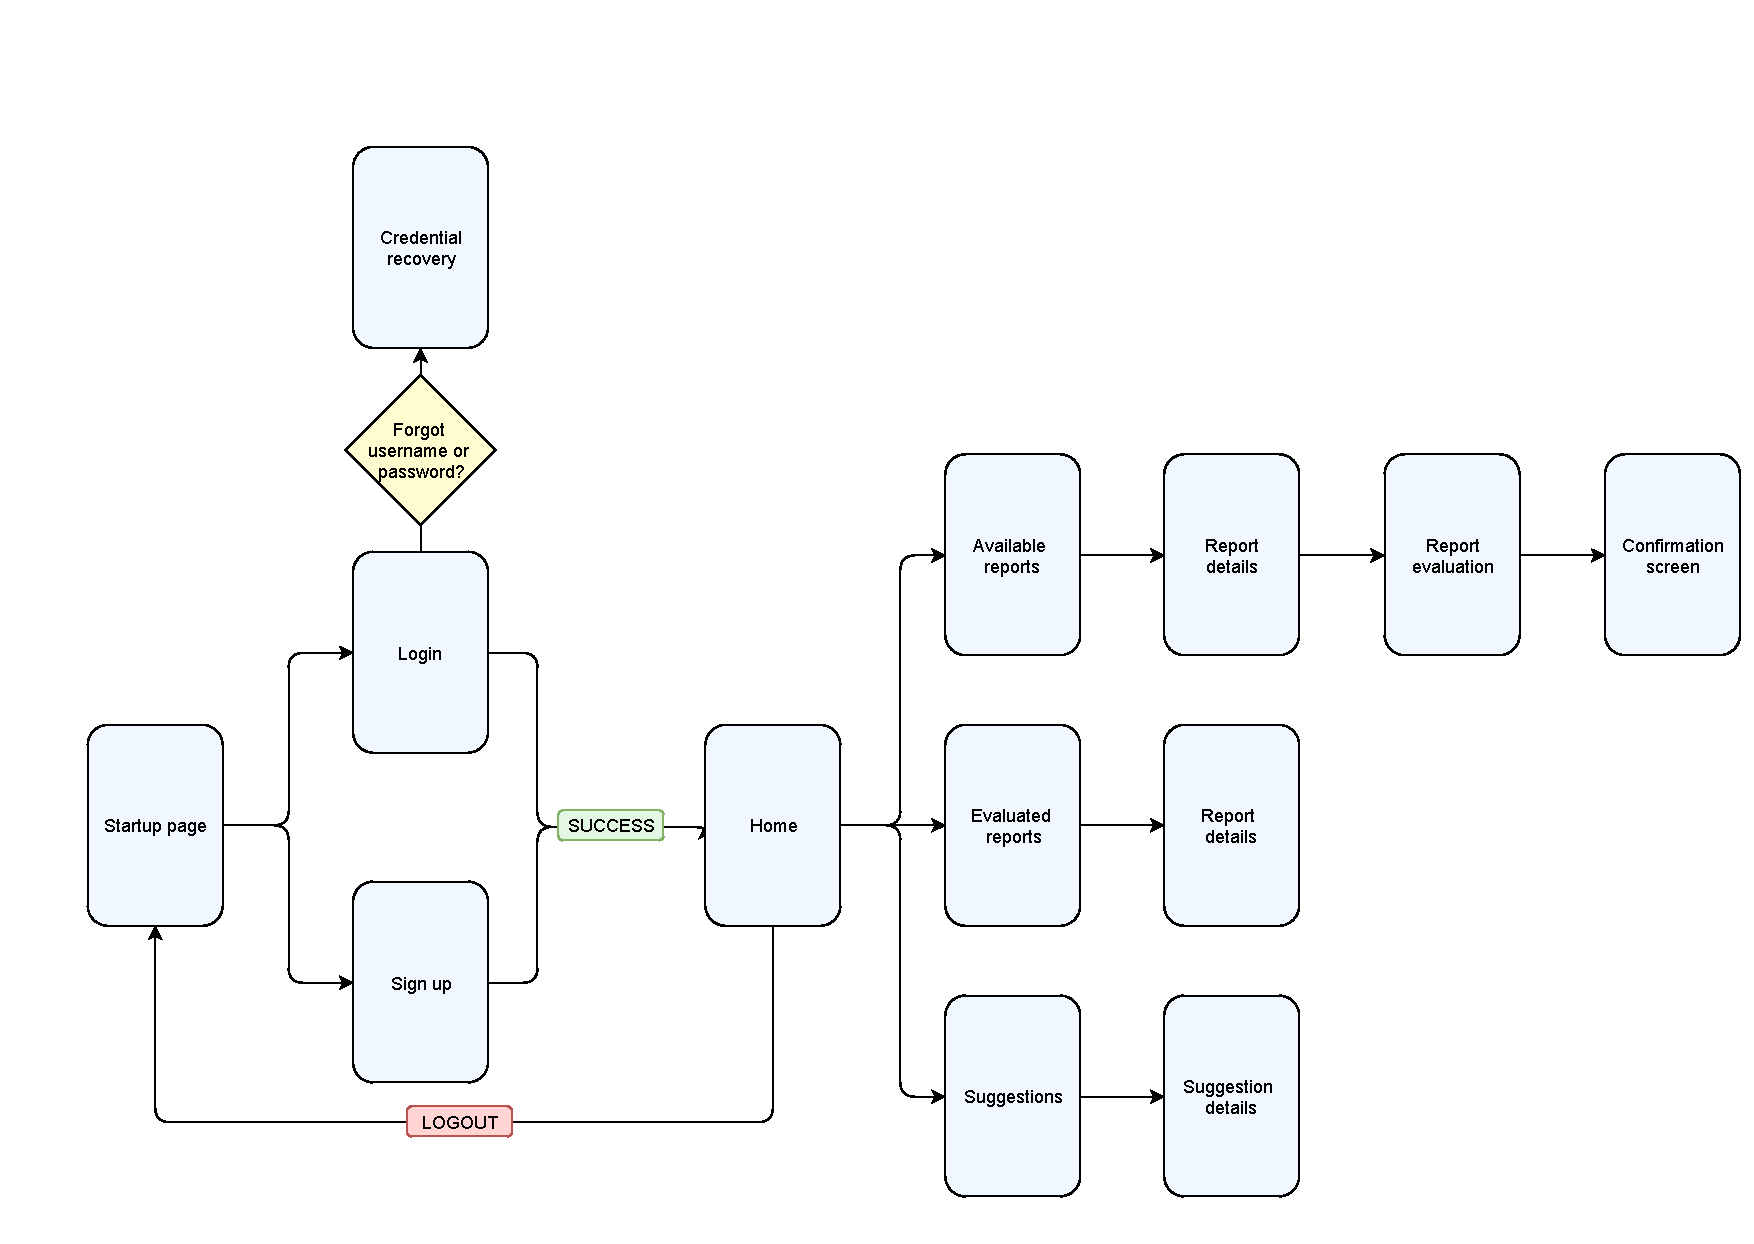
\includegraphics[scale = 0.65, center]{authorityux}
				\caption{}
		\end{figure}
	%end of third chapter

	\chapter{Requirements Traceability}
	%end of fourth chapter

	\chapter{Implementation, Integration and Test plan}
	%end of fiveth chapter

	\chapter{Effort Spent}
		\begin{table}[H]
		\centering
		\begin{tabular}{|c|c|c|}
			\hline
			Chapter & Frangi (hours) & Fucci (hours)\\
			\hline
			\hline
			Chapter 1 & ? & ?\\
			\hline
			Chapter 2 & ? & ?\\
			\hline
			Chapter 3 & ? & ?\\
			\hline
			Chapter 4 & ? & ?\\
			\hline
			Chapter 5 & ? & ?\\
			\hline
			Total hours: & ? & ?\\
			\hline
		\end{tabular}
		\label{tab: }
	\end{table}
	%end of sixth chapter
	\chapter{References}
	%end of seventh chapter
\end{document}